%----------------------------------------------
% PACCHETTI
%----------------------------------------------
\documentclass[12pt,a4paper]{article}
\usepackage[a4paper]{geometry}
\usepackage[T1]{fontenc}
\usepackage[utf8]{inputenc}
\usepackage[italian]{babel}
\usepackage{lipsum}
\usepackage{hyperref}
\usepackage{lastpage}
\usepackage{fancyhdr}
\usepackage{graphicx}
\usepackage{url}
\usepackage{geometry}
\usepackage{xcolor}
\usepackage{amssymb}
\usepackage{amsmath}
\usepackage{booktabs}

%----------------------------------------------
% NUOVI COMANDI
%----------------------------------------------
\newcommand{\Sep}{\vspace{1.5em}}
\newcommand{\MidSep}{\vspace{1em}}
\newcommand{\SmallSep}{\vspace{0.5em}}

\newcommand{\numberset}{\mathbb}
\newcommand{\N}{\numberset{N}} 
\newcommand{\Z}{\numberset{Z}}
\newcommand{\Q}{\numberset{Q}}
\newcommand{\R}{\numberset{R}}
\newcommand{\C}{\numberset{C}}
%----------------------------------------------
% INTESTAZIONE  E PIE DI PAGINA
%----------------------------------------------
\pagestyle{myheadings}
\pagestyle{fancy}
\fancyhf{}
\hypersetup{hidelinks}

\headsep= 20mm

\renewcommand{\headrulewidth}{2pt}
\renewcommand{\footrulewidth}{2pt}

\lhead{
\includegraphics[width=0.4\columnwidth]{../../img/units_logo.png}}
\rhead{
\includegraphics[width=0.3\columnwidth]{../../img/logo_black.png}}\lfoot{Copyright © Enrico Lacchin | \url{www.enricolacchin.com}}
\cfoot{}
\rfoot{\thepage}

\leftskip 0.0pt
\usepackage[utf8]{inputenc}
\usepackage{amsmath}
\usepackage{amssymb}
\usepackage{xcolor}
\usepackage{listings}
\usepackage{xstring}

\definecolor{dkgreen}{rgb}{0,0.6,0}
\definecolor{ltgray}{rgb}{0.5,0.5,0.5}
\definecolor{royalpurple}{rgb}{0.47, 0.32, 0.66}

\makeatletter
\newif\ifcolname
\colnamefalse

\def\keywordcheck{%
\IfStrEq*{\the\lst@token}{SELECT}{\global\colnametrue}{}%
\IfStrEq*{\the\lst@token}{WHERE}{\global\colnametrue}{}%
\IfStrEq*{\the\lst@token}{FROM}{\global\colnamefalse}{}%
\IfStrEq*{\the\lst@token}{USE}{\global\colnamefalse}{}%
\color{orange}%
}
\def\setidcolor{%
\ifcolname\color{royalpurple}\else\color{black}\fi%
}
\makeatother

\lstset{
    basicstyle={\small\ttfamily},
    breakatwhitespace=false,
    breaklines=true,
    captionpos=b,
    commentstyle=\color{dkgreen},
    deletekeywords={...},
    escapeinside={\%*}{*)},
    extendedchars=true,
    frame=single,
    keepspaces=true,
    language=SQL,
    otherkeywords={IS, IF, SHOW, DECLARE, OPEN, FETCH, CLOSE, DATABASE, DATABASES, USE, COMMENT, CHANGE, REFERENCES, RENAME, TO, IS, AUTO_INCREMENT, EXISTS},
    morekeywords={*,modify,MODIFY,...},
    keywordstyle=\keywordcheck,
    identifierstyle=\setidcolor,
    stringstyle=\color{red},
    numbers=left,
    numbersep=15pt,
    numberstyle=\tiny,
    rulecolor=\color{ltgray},
    showspaces=false,
    showstringspaces=false, 
    showtabs=false,
    stepnumber=1,
    tabsize=2,
    xleftmargin =1em
}

%----------------------------------------------
% INIZIO DOCUMENTO
%----------------------------------------------
\begin{document}

%----------------------------------------------
% TITOLO
%----------------------------------------------
\pagenumbering{gobble}

\small{Enrico Lacchin}

\MidSep
\textbf{\LARGE{Progetto Finale}}

\MidSep
\textit{\Large{079IN - Basi di Dati}}
\Sep

\begin{center}

\includegraphics[width=1\columnwidth]{../../img/db}
\end{center}

\vfill
Corso: 079IN - Basi di Dati

Docente: De Lorenzo Andrea

Consegna: 30 Maggio 2023

%----------------------------------------------
% INDICE
%----------------------------------------------

\clearpage
\pagenumbering{roman}
\setcounter{page}{1}
\tableofcontents

%----------------------------------------------
% INIZIO CAPITOLI
%----------------------------------------------
% NUOVO CAPITOLO
\clearpage

\pagenumbering{arabic}
\setcounter{page}{1}

\section{Presentazione Progetto}\label{sec:presentazione-progetto}
Si vuole realizzare un database per la COMPANY LTD, società che opera nel mondo dell’organizzazione degli eventi, nella comunicazione online (siti web, social media, advertising, etc. \dots ) e svolge alcune operazioni nel mondo dell’aviazione. La società necessita un database relazionale per gestire tutte le operazioni e i progetti che svolgono quotidianamente. Spesso la società si appoggia a fornitori esterni e collaboratori e questi dovranno essere rappresentati con delle tabelle.

\subsection{Requisiti del Database}\label{subsec:requisiti-del-database}
\begin{itemize}
\item Per ogni dipendente deve esserci una relazione con il suo superiore, con il suo dipartimento di competenza e dev'essere indicato se fa parte del Consiglio di Amministrazione.
\item Ad ogni progetto devono essere assegnati un cliente, una fattura (inizialmente può non esserci), un dipartimento di competenza e i fornitori necessari per quel progetto.
\item Per ogni cliente ci deve essere il dipartimento di riferimento.
\item Ogni dipartimento deve avere un riferimento a un ufficio e ad un manager.
\item Ogni fornitore/collaboratore deve avere un dipartimento di competenza.
\item Ogni cliente e fattura deve avere uno stato compreso in una lista specifica.
\item Ogni dipendente deve far riferimento ad almeno un dipartimento.
\end{itemize}

\subsection{Azioni del Database}\label{subsec:azioni-del-database}
La COMPANY LTD dovrà svolgere le seguenti azioni sul database:
\begin{itemize}
\item Una volta all'anno viene richiesta la visione di tutti i membri nel direttivo per convocare il CdA
\item Un volta al giorno vengono aggiornati i progetti e le fatture ed eventualmente aggiunti clienti, fornitori e collaboratori
\item Una volta all'anno vengono visualizzate tutte le fatture emesse nel corso dell'anno e il fatturato totale per poter redigere il bilancio
\item In base all'andamento dell'azienda ci deve essere la possibilità di aggiungere dipartimenti e/o uffici
\item Due volte all'anno la COMPANY LTD vuole sapere a quali clienti sono state rilasciate $N$ o più fatture (dal 1 gennaio dell'anno in corso).
\item L'azienda ha il bisogno di vedere le fatture emesse tra due date specifiche per monitorare l'andamento.
\end{itemize}

% NUOVO CAPITOLO
\section{Schema Entity - Relationship}\label{sec:schema-entity---relationship}
\begin{center}
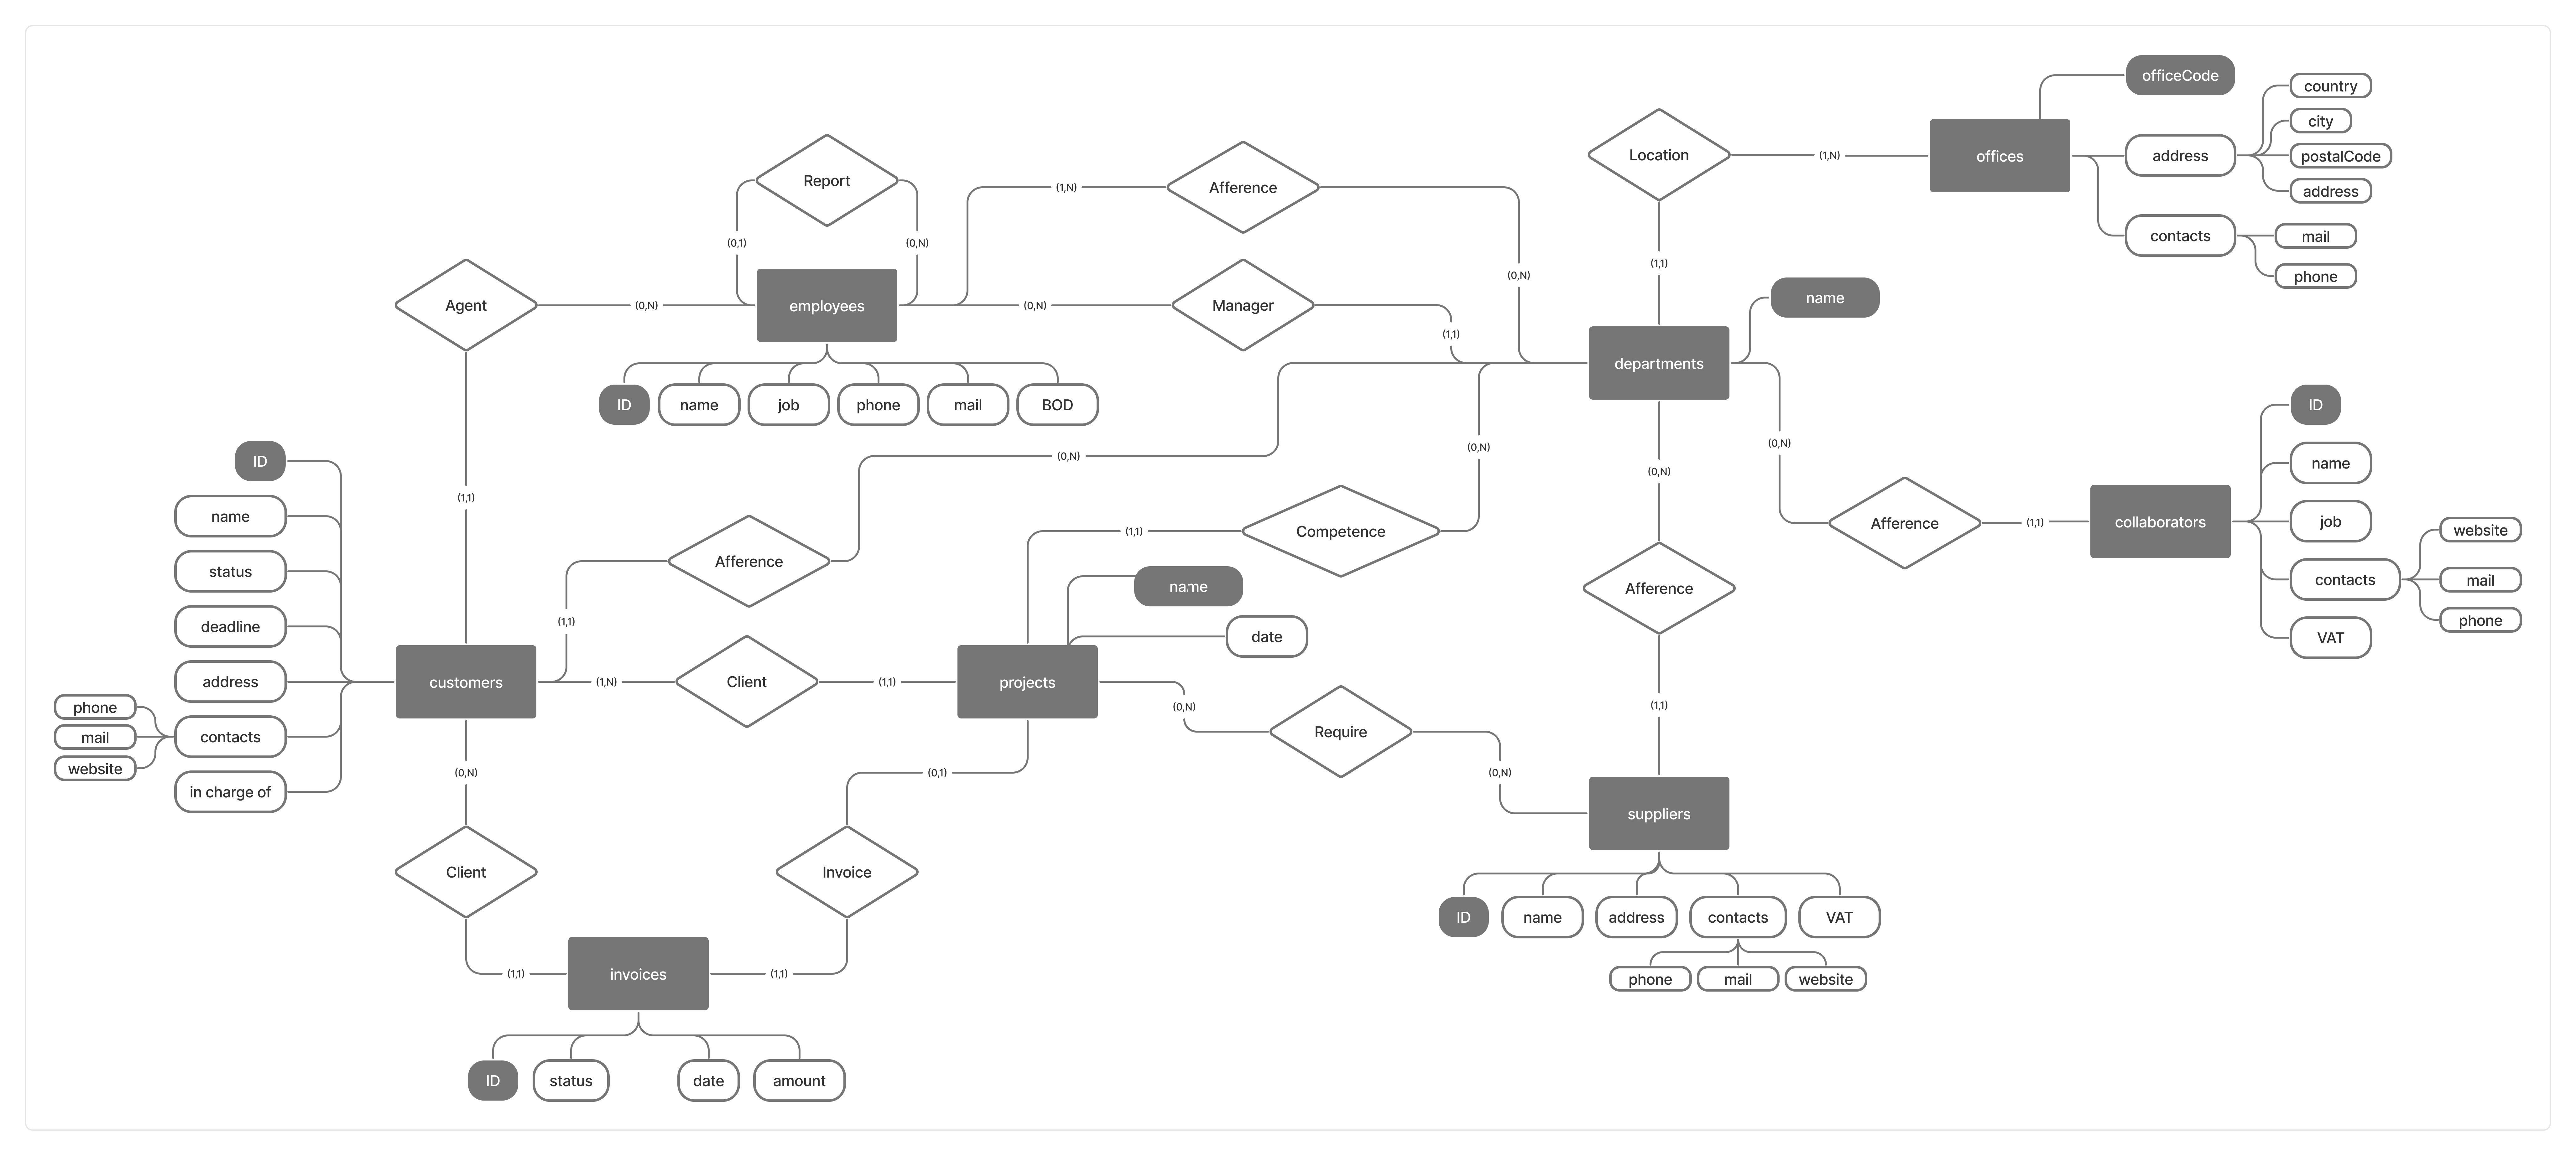
\includegraphics[width=0.9\columnwidth]{../../img/er_scheme}
\end{center}


% NUOVO CAPITOLO
\section{Dizionario dei Dati}\label{sec:dizionario-dei-dati}
\subsection{Entità}\label{subsec:entita}
\resizebox{\textwidth}{!}{%
\begin{tabular}{|l|l|l|l|}
\hline
\multicolumn{1}{|c|}{\textbf{Entità}} & \multicolumn{1}{c|}{\textbf{Descrizione}} & \multicolumn{1}{c|}{\textbf{Attributi}} &  \multicolumn{1}{c|}{\textbf{Identificatore}}\\ \hline \hline
\textit{Customers} & Clienti dell’azienda & ID, nome, stato, fine dell’accordo, indirizzo, contatti, agente& ID \\
\textit{Employees} & Dipendenti dell’azienda & ID, nome, ruolo, telefono, mail, flag se sono nel CdA & ID \\
\textit{Projects} & Lista dei progetti svolti dall’azienda & Nome, data & nome \\
\textit{Invoices} & Lista delle fatture emesse & ID, stato, data di emissione, prezzo & ID \\
\textit{Departments} & Lista dei dipartimenti dell’azienda & Nome & nome \\
\textit{Suppliers} & Lista dei fornitori dell’azienda & ID, nome, indirizzo, contatti, p. IVA & ID \\
\textit{Collaborators} & Persone/Aziende che collaborano con la  COMPANY LTD & ID, nome, lavoro, contatti, p. IVA & ID \\
\textit{Offices} & Uffici dell’azienda & Codice ufficio, indirizzo, contatti &  \\ \hline
\end{tabular}%
}

\subsection{Relationship}\label{subsec:relationship}
\resizebox{\textwidth}{!}{%
\begin{tabular}{|l|l|l|}
\hline
\multicolumn{1}{|c|}{\textbf{Relazione}} & \multicolumn{1}{c|}{\textbf{Descrizione}} & \multicolumn{1}{c|}{\textbf{Componenti}} \\ \hline \hline
\textit{Agente} & Dipendente responsabile del cliente & Clienti, dipendenti \\
\textit{Report} & Persona di riferimento per il dipendente & Dipendenti \\
\textit{Manager} & Manager del dipartimento & Dipendenti, dipartimenti \\
\textit{Cliente} & Cliente relativo a un progetto & Progetti, clienti \\
\textit{Cliente} & Cliente relativo a una fattura & Fatture, clienti \\
\textit{Fattura} & Fattura relativa al progetto & Fatture, progetti \\
\textit{Richiede} & Necessità o meno di fornitori per un progetto & Fornitori, progetti \\
\textit{Competenza} & Dipartimento di competenza per un progetto & Progetti, dipartimenti \\
\textit{Locazione} & Sede principale del dipartimento & Uffici, dipartimenti \\
\textit{Afferisce} & Dipartimento di riferimento per il collaboratore & Dipartimenti, collaboratori \\
\textit{Afferisce} & Dipartimento di riferimento per il fornitore & Dipartimenti, fornitori \\
\textit{Afferisce} & Dipartimento di riferimento per il dipendente & Dipartimenti, dipendenti \\
\textit{Afferisce} & Dipartimento di riferimento per il cliente & Dipartimenti, clienti\\ \hline
\end{tabular}%
}

% NUOVO CAPITOLO
\section{Vincoli non esprimibili}\label{sec:vincoli-non-esprimibili}
Dall'analisi dei requisiti dei database si evincono i seguenti vincoli non esprimibili:
\begin{itemize}
\item Lo stato delle fatture deve essere compreso in una lista, che successivamente definiremo come: Draft, Not Paid e Paid
\item Lo stato del cliente dev'essere compreso in una lista, che successivamente definiremo come: Ongoing Negotiation, Agreed, In Progress e Done
\item La colonna dove si determina se il dipendente è nel CdA o meno (colonna BOD) può avere solo valore VERO (T) o FALSO (F)
\end{itemize}

% NUOVO CAPITOLO
\section{Tavola dei volumi}\label{sec:tavola-dei-volumi}
Si suppone che la COMPANY LTD sia una PMI con: 
\begin{itemize}
\item 100 dipendenti
\item 10 dipartimenti
\item 10 uffici
\item 500 clienti
\item 100 fornitori
\item 20 collaboratori
\item 1000 fatture emesse all'anno relative a 1000 progetti
\item 4 fornitori ogni 10 progetti (400 fornitori per 1000 progetti)
\end{itemize}
Ne segue quindi la Tavola dei volumi:

\begin{center}
\begin{tabular}{|l|l|l|}
\hline
\multicolumn{1}{|c|}{\textbf{Concetto}} & \multicolumn{1}{c|}{\textbf{Tipo}} & \multicolumn{1}{c|}{\textbf{Volume}} \\ \hline \hline
\textit{Dipendente} & E & 100 \\
\textit{Ufficio} & E & 10 \\
\textit{Dipartimento} & E & 10 \\
\textit{Cliente} & E & 500 \\
\textit{Collaboratore} & E & 20 \\
\textit{Fornitore} & E & 100 \\
\textit{Fattura} & E & 1000 \\
\textit{Progetto} & E & 1000 \\
\textit{Richiede} & R & 400\\ \hline
\end{tabular}\end{center}
Ho omesso nella tabella dei volumi molte relazioni, poiché facilmente calcolabili dai volumi delle entità.

% NUOVO CAPITOLO 
\section{Analisi delle ridondanze}\label{sec:analisi-delle-ridondanze}
Per migliorare lo schema Entity - Relationship sono andato ad analizzare tutti i cicli presenti per vedere se poteva essere eliminata qualche relazione superflua.\\
\\
\textbf{Cicli analizzati}:\\
\\
\textbf{\textit{Customers - Projects - Invoices}}:
\begin{center}
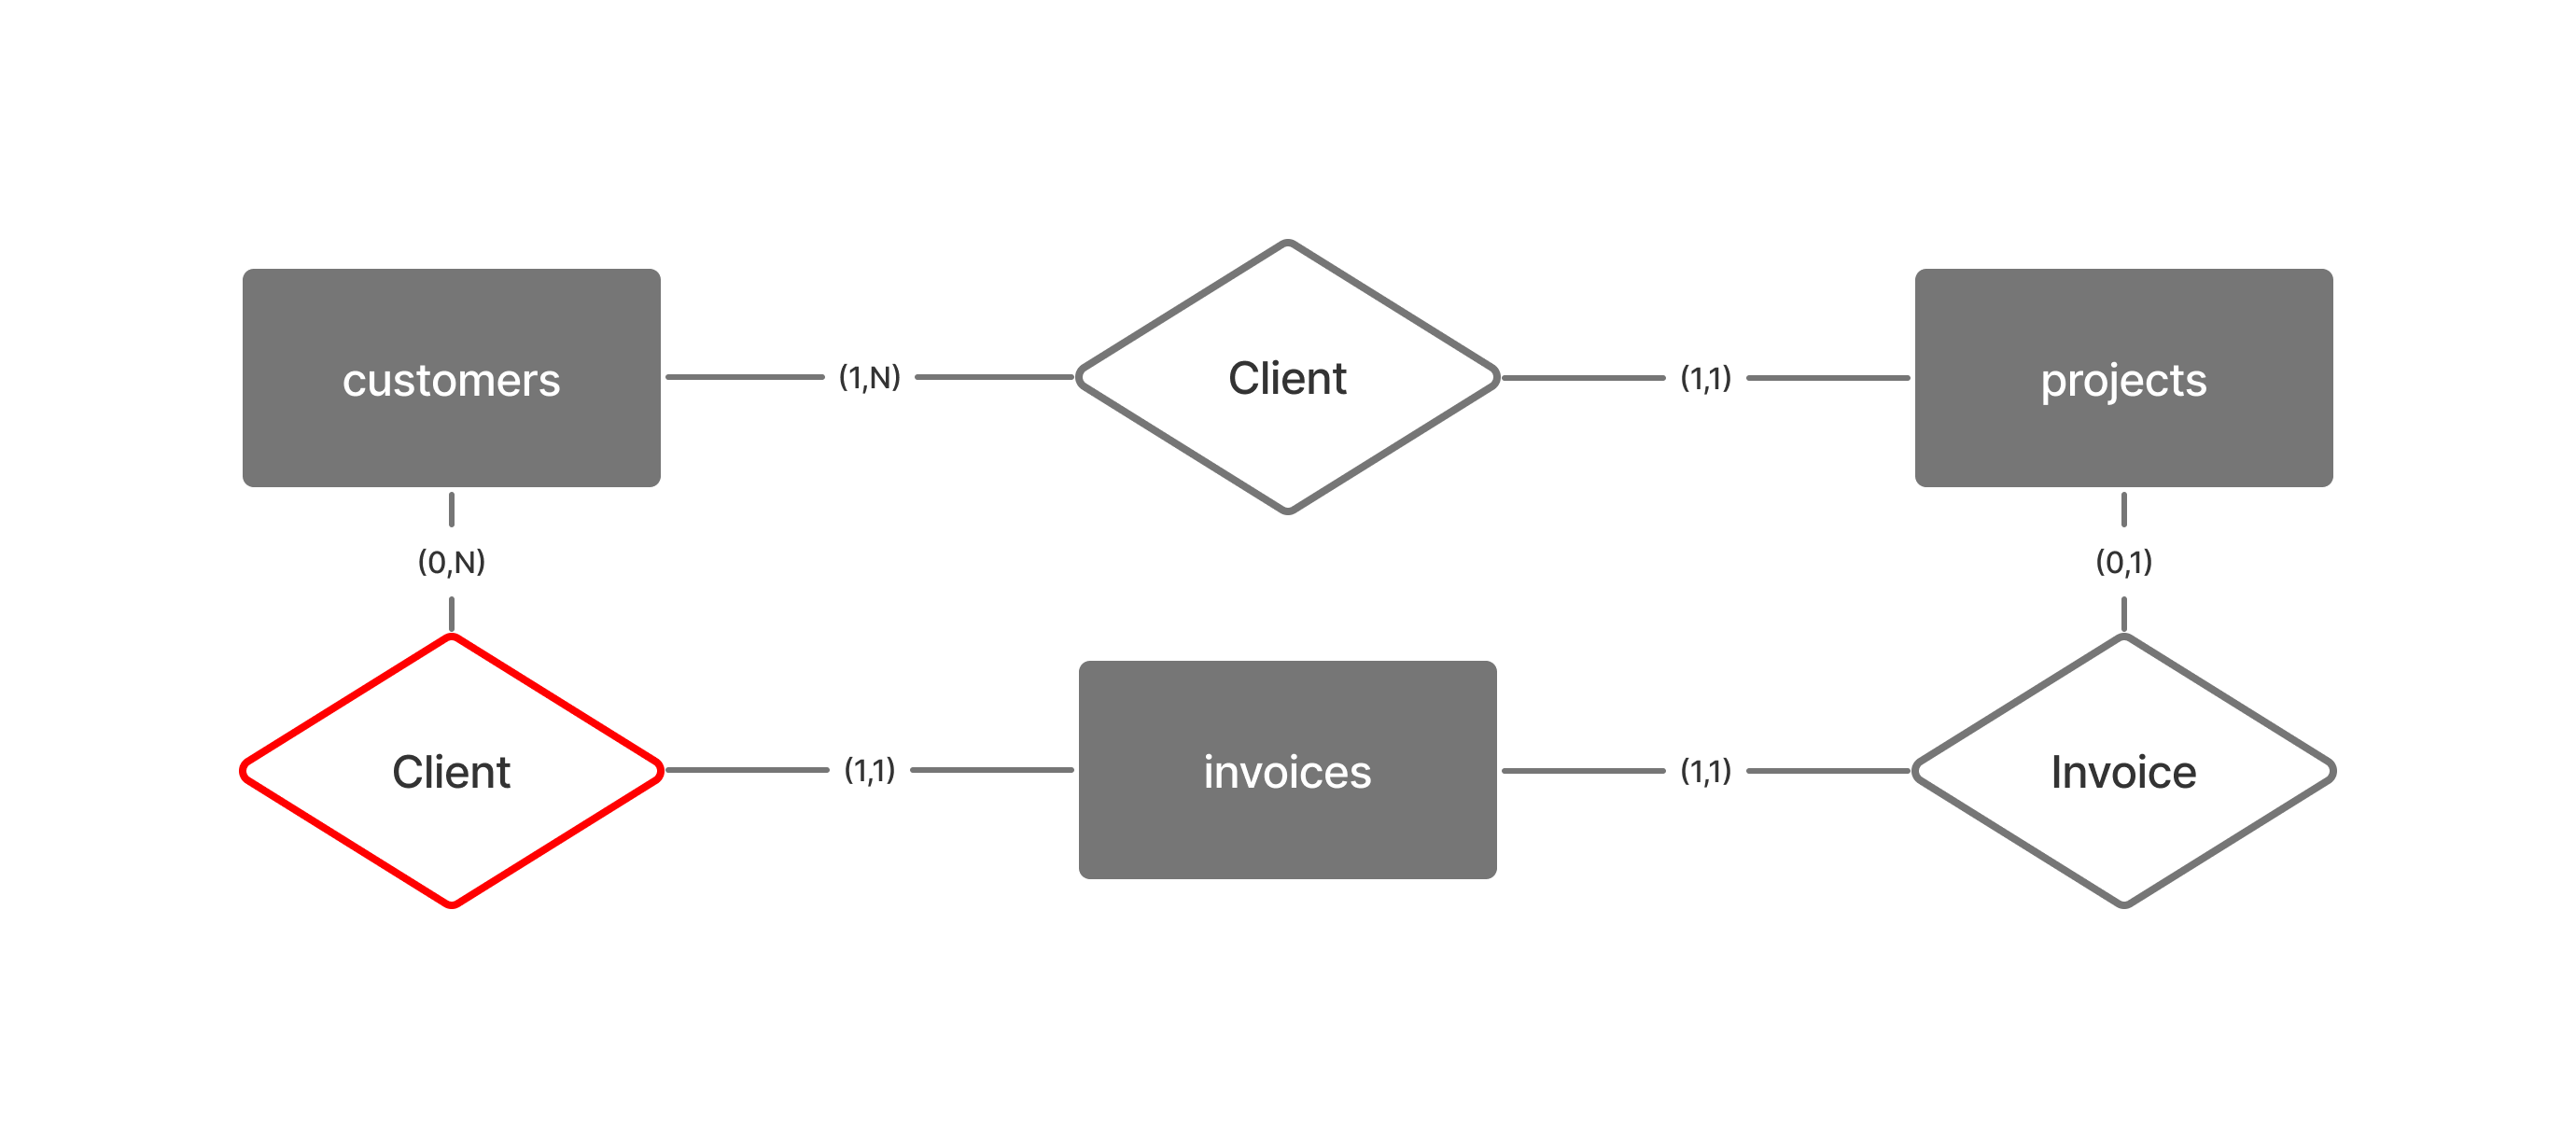
\includegraphics[width=0.6\columnwidth]{../../img/er_cycle_custumers-projects-invoices}
\end{center}
In particolare vado ad analizzare la ridondanza della relazione "Client" identificata dal colore \textcolor{red}{rosso}.
Noto che la relazione "Client" tra le entità "projects" e "customers" è obbligatoria (cardinalità $(1,1)$) di conseguenza, se si vuole visionare il cliente di una determinata fattura, si potrebbe ricavare facilmente guardando il progetto relativo.\\
\\
In conclusione quella relazione può essere eliminata e nella tabella "invoices" non ci sarà la voce "client" ma solamente il progetto relativo a quella fattura.\\
\\
\\
\textbf{\textit{Customers - Employees - Departments}}:
\begin{center}
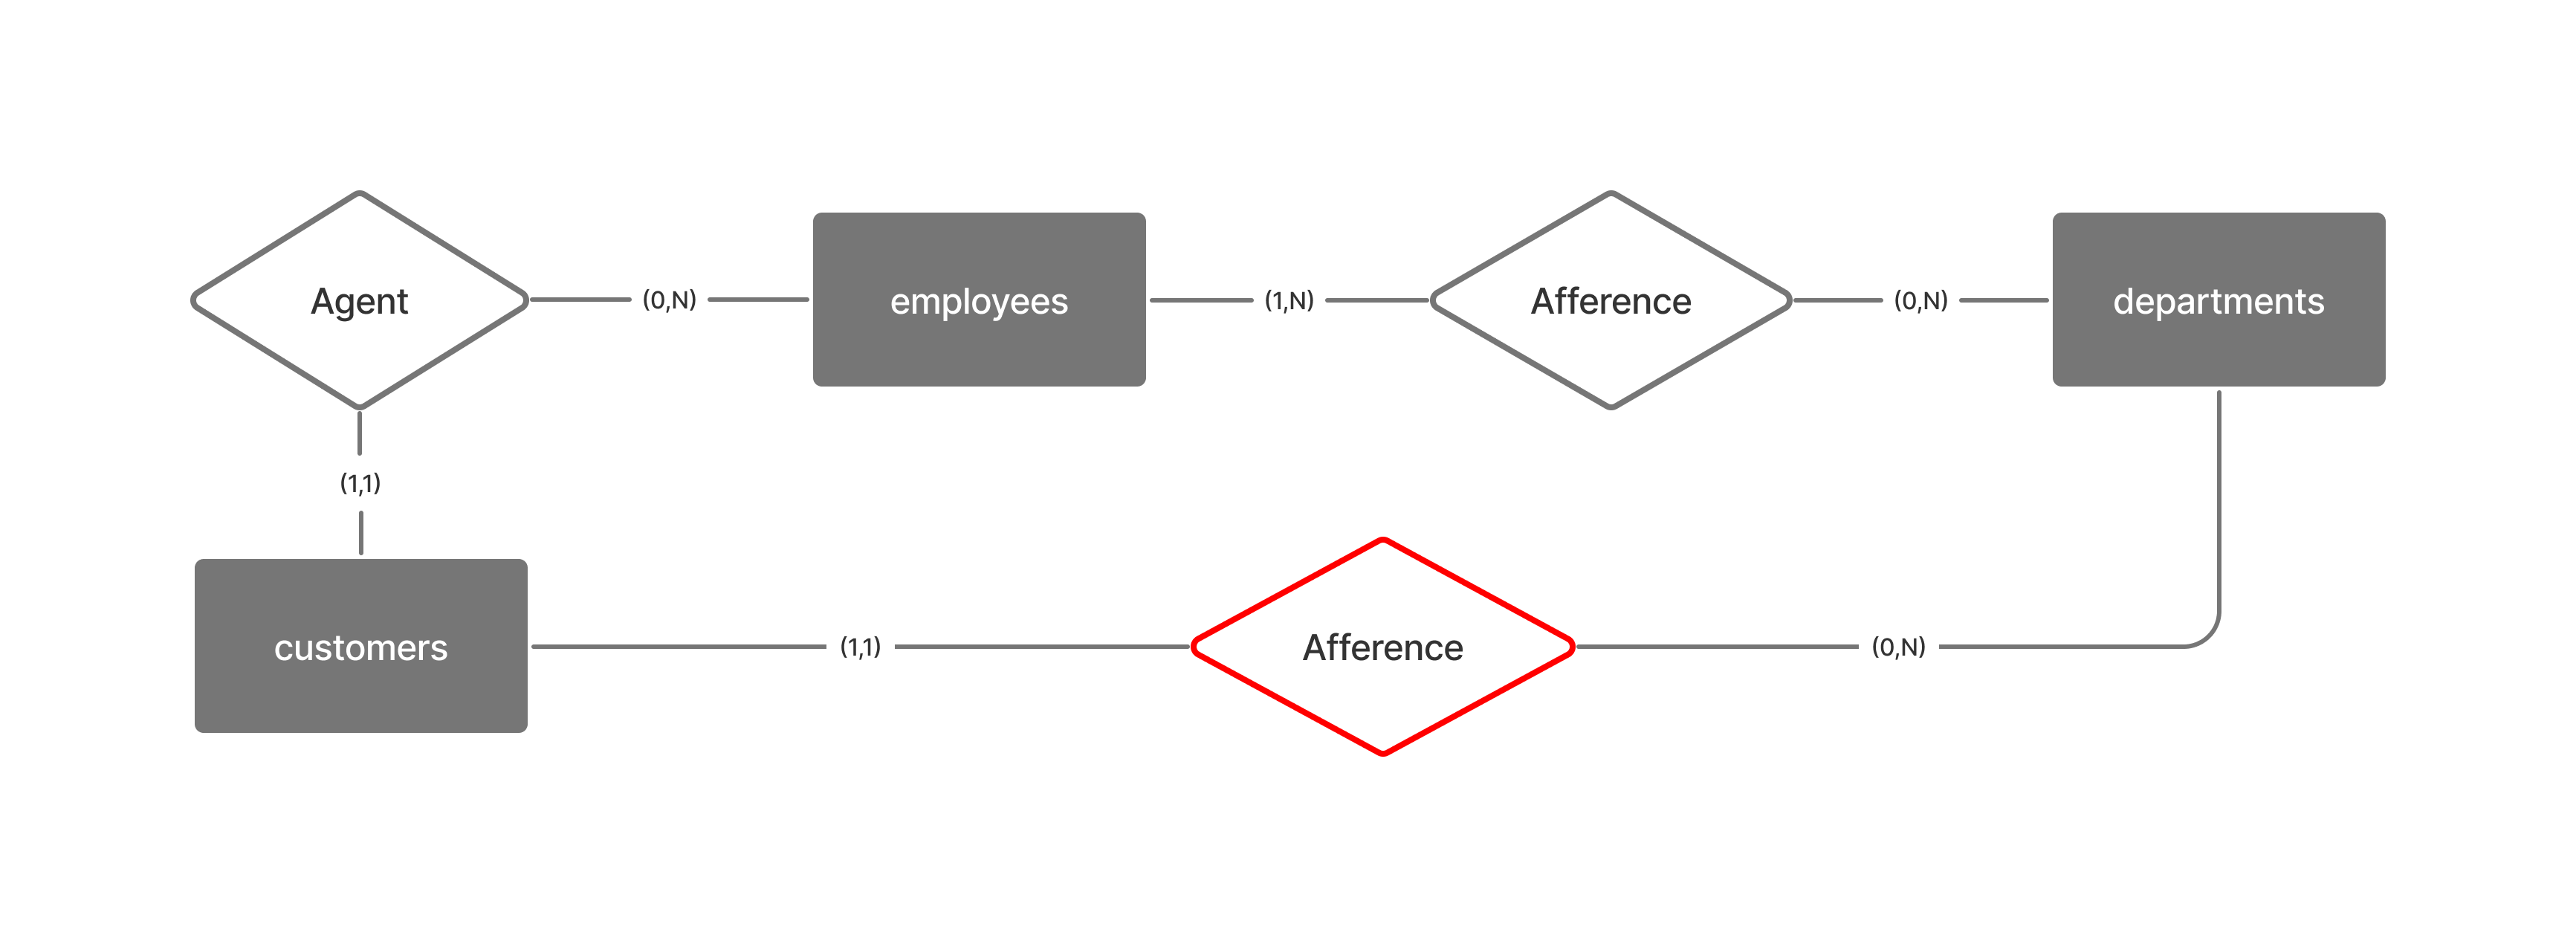
\includegraphics[width=0.6\columnwidth]{../../img/er_cycle_customers-employees-departments}
\end{center}
In questo caso vado ad analizzare la ridondanza "Afference" sempre identificata in \textcolor{red}{rosso}.
Dallo schema ER si evince che ogni dipendente dev'essere assegnato un dipartimento e che ad ogni cliente dev'essere assegnato un agente. Da questa analisi si potrebbe dire "\textit{posso ricavare il dipartimento del cliente da quello dell'agente}".\\
\\
Se, però, andiamo a vedere la cardinalità tra employees $\rightarrow$ Afference $\rightarrow$ departments notiamo che è uguale a $(1,N)$ ossia che un dipendente può far riferimento a $1$ o $N$ dipartimenti quindi, in determinati casi, non saprei identificare un dipartimento specifico.\\
\\
In conclusione la relazione "Afference" tra "customers" e "departments" non risulta duplicata ma bensì necessaria, anche considerando il fatto cha altrimenti si violerebbe uno dei requisiti del database.\\
\\
\\
\textbf{\textit{Projects - Departments - Suppliers}}:
\begin{center}
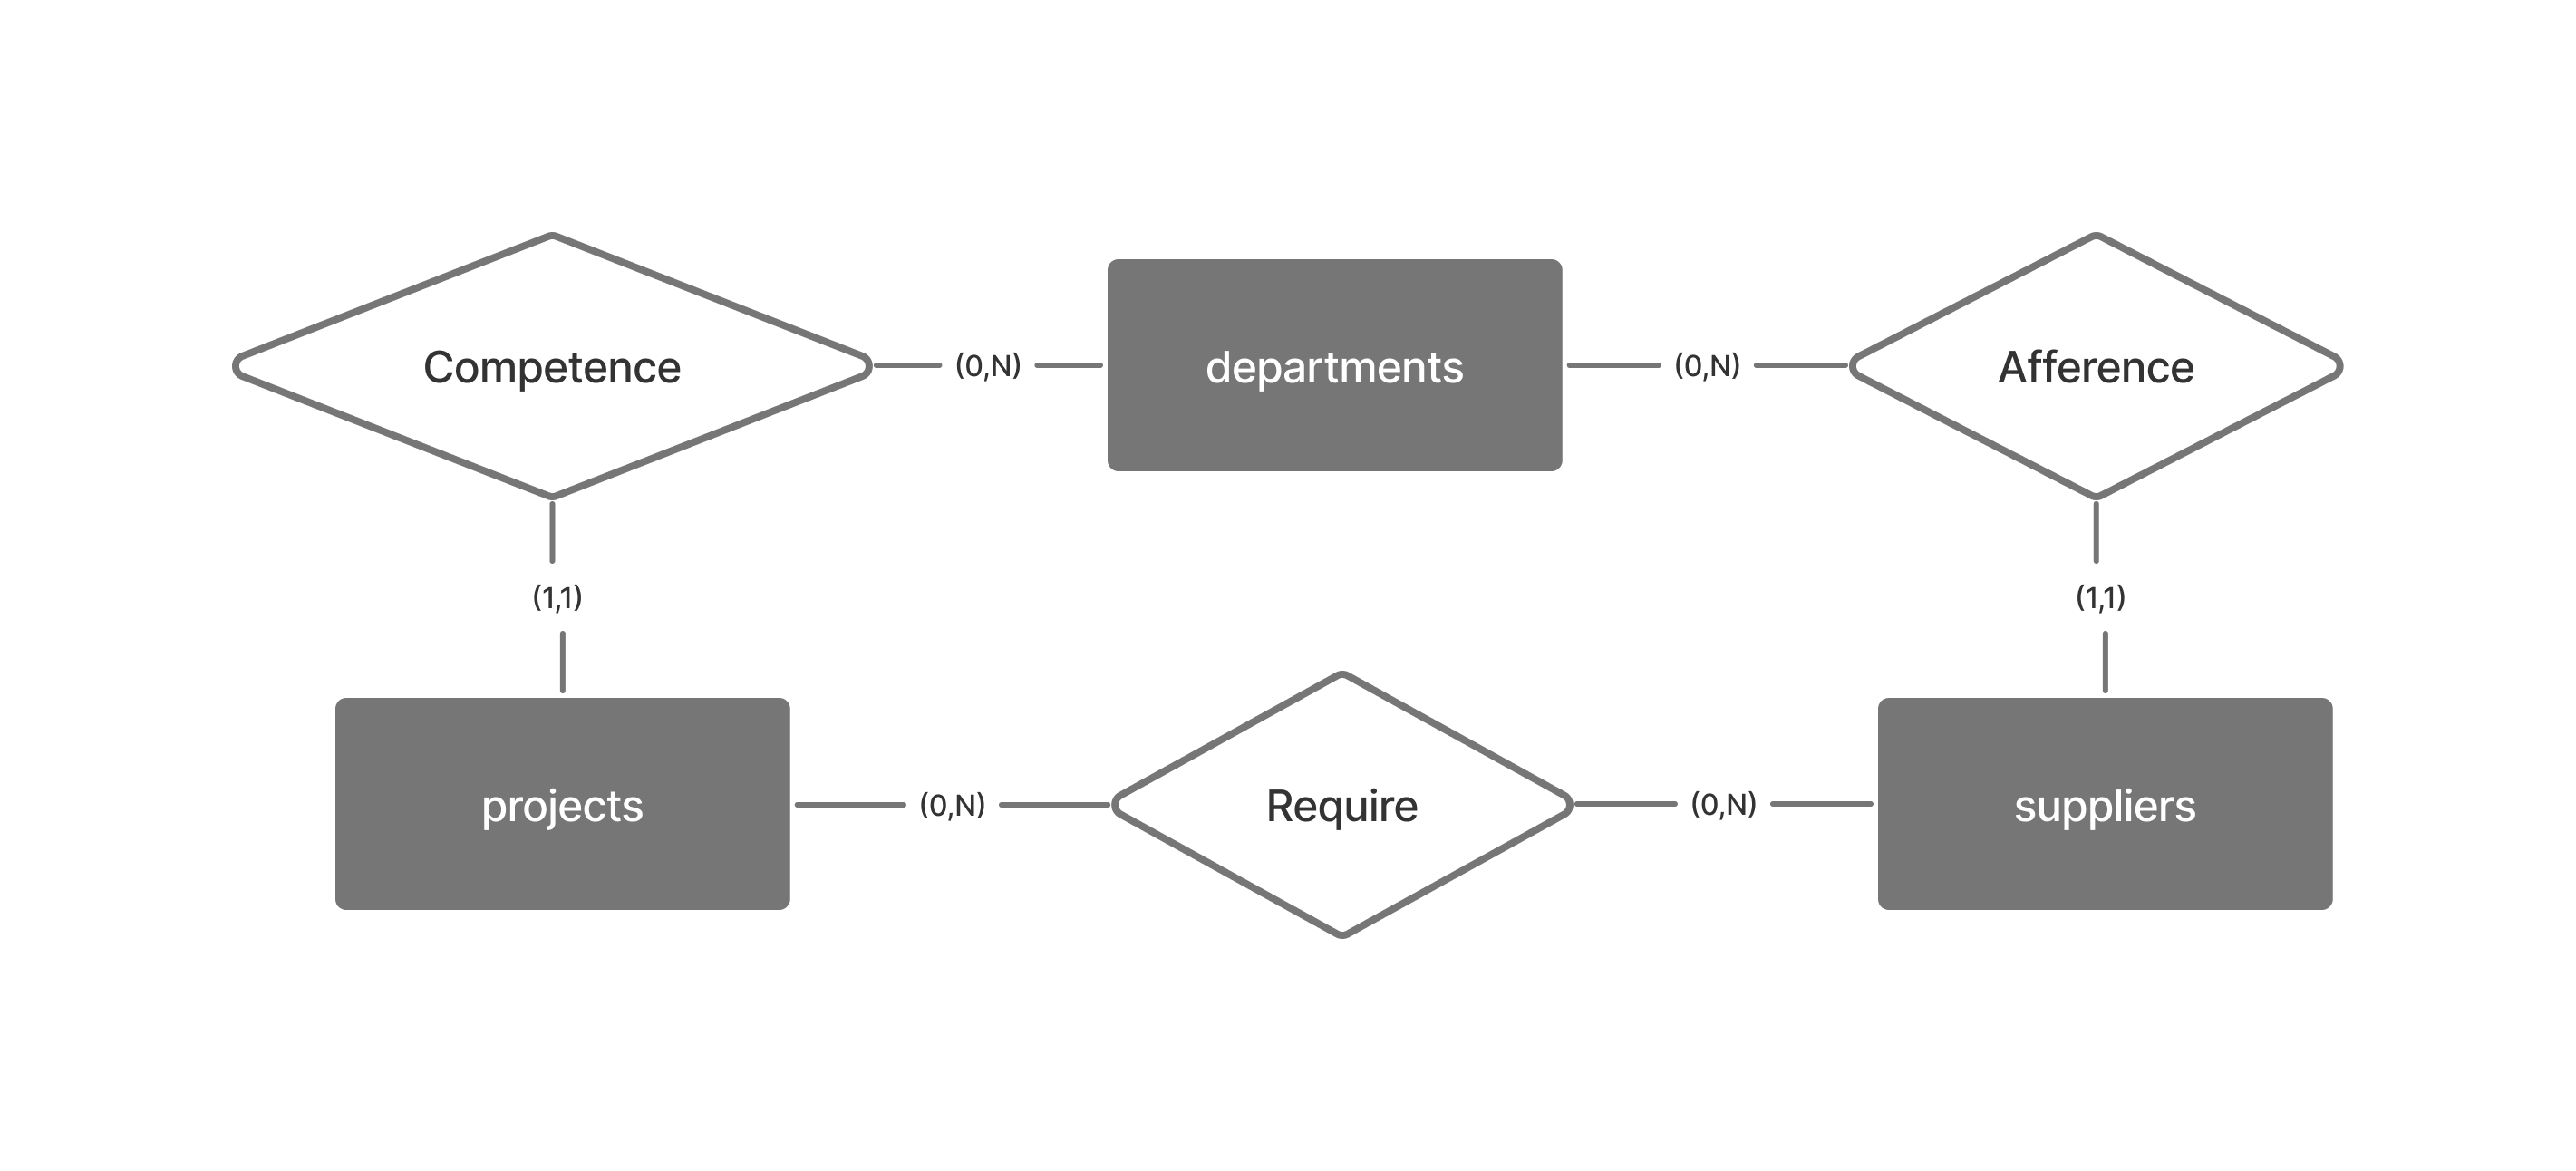
\includegraphics[width=0.6\columnwidth]{../../img/er_cycle_projects-departments-suppliers}
\end{center}
In questo ciclo non risulta nessuna ridondanza poiché ad ogni progetto e ad ogni fornitore deve essere assegnato un dipartimento ma non è detto che in ogni progetto siano necessari fornitori (vista la cardinalità $(0,N)$).\\
\\
Ne consegue che la relazione projects $\rightarrow$ Require $\rightarrow$ suppliers non è ridondante anche vista la sua natura di relazione "molti a molti".\\
\\
\\
\textbf{\textit{Customers - Departments - Projects}}:
\begin{center}
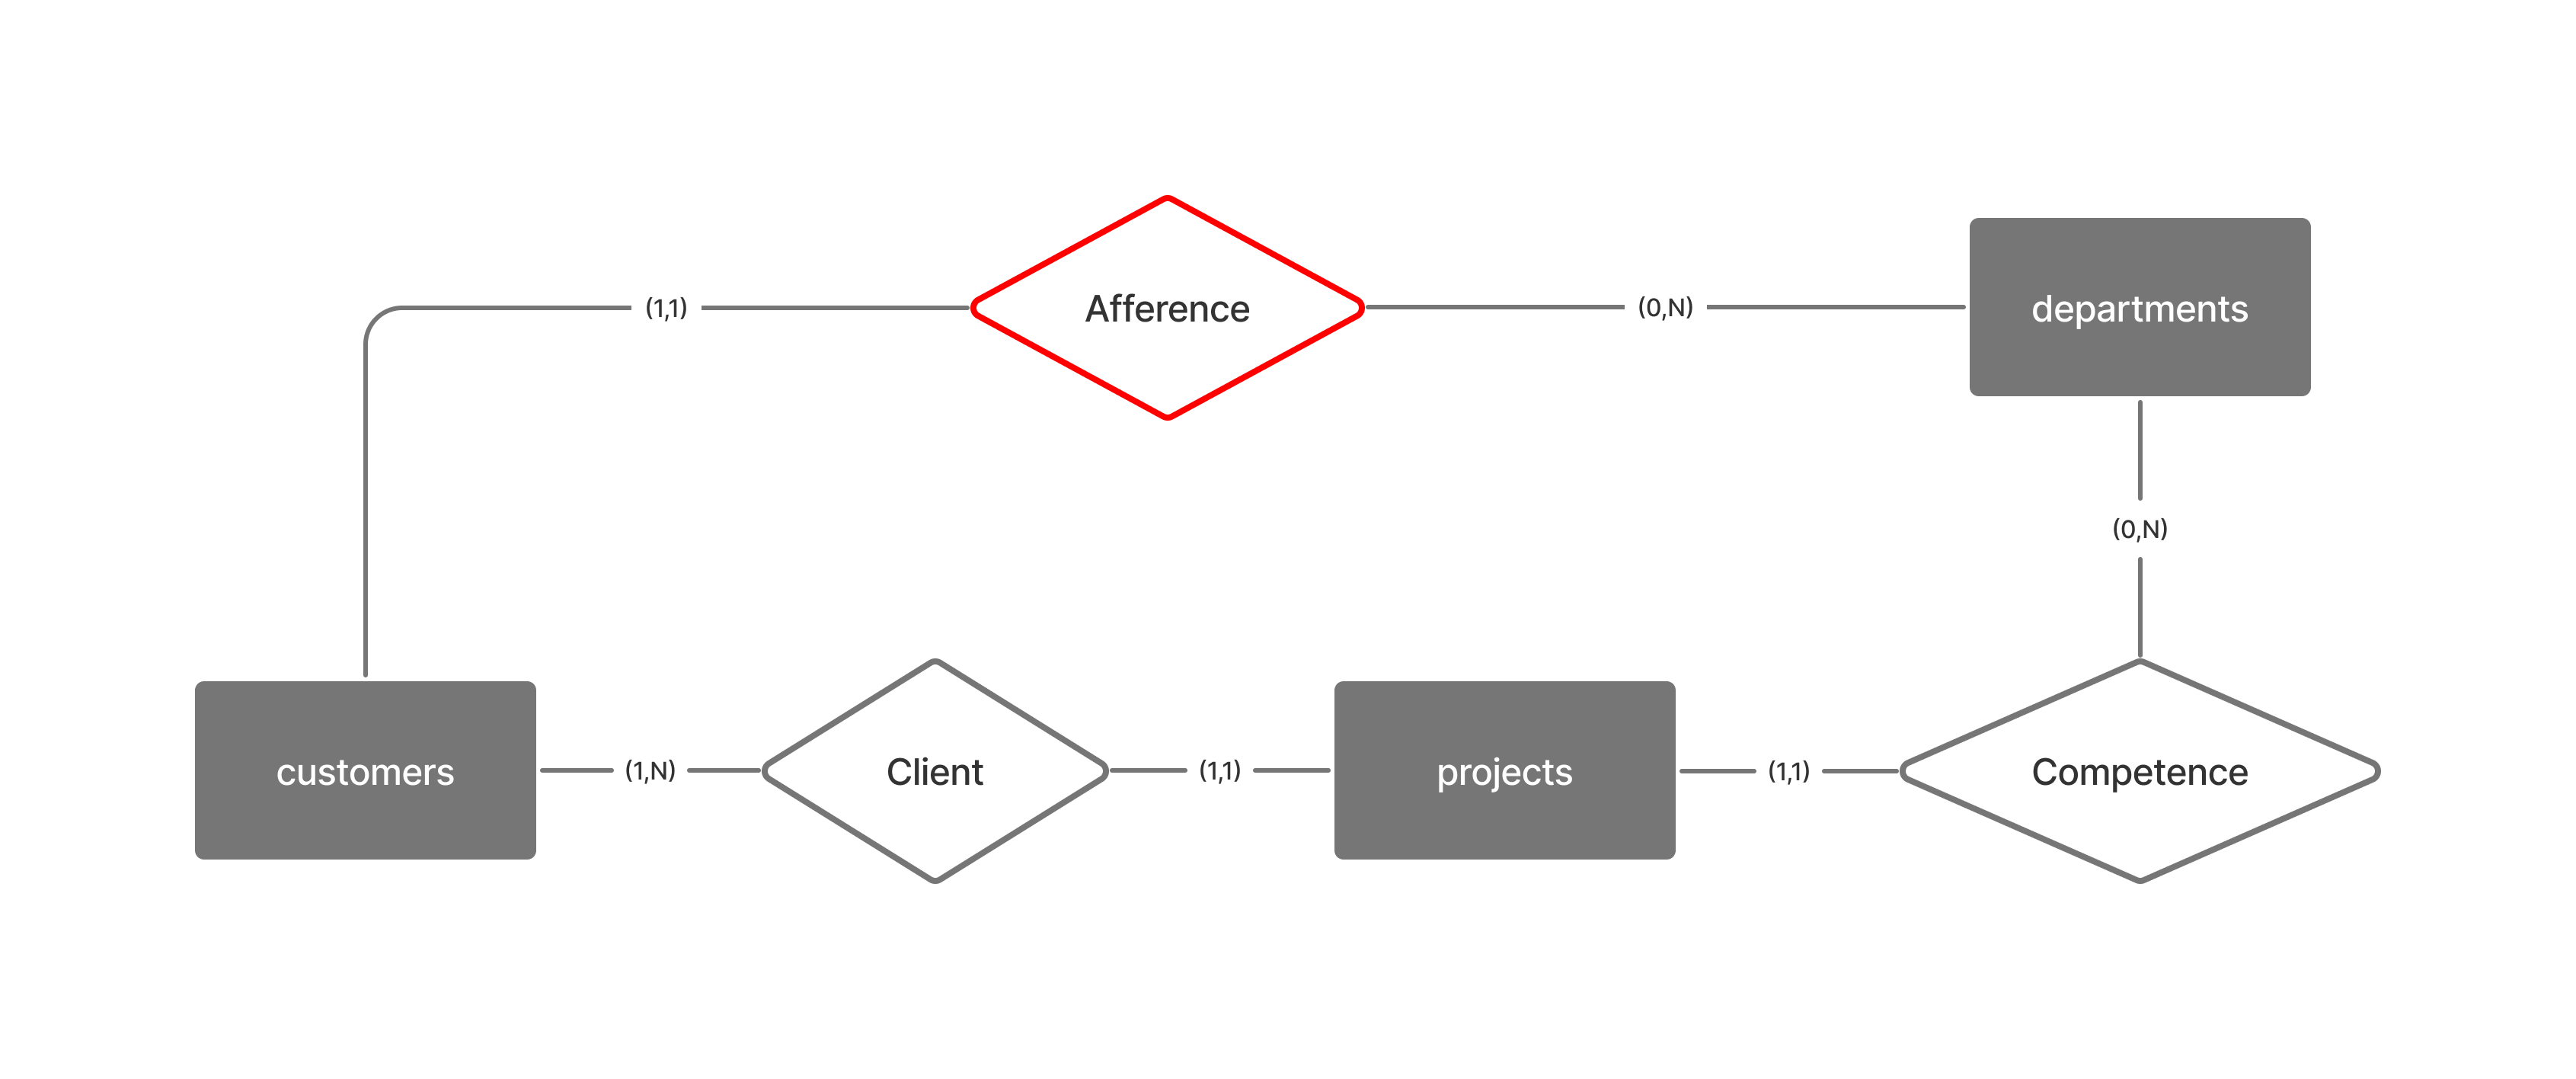
\includegraphics[width=0.6\columnwidth]{../../img/er_cycle_customers-departments-projects}
\end{center}
In questo ciclo voglio analizzare se posso rimuovere la relazione "Afference" tra "customers" e "departments" evidenziata in \textcolor{red}{rosso}.\\
\\
Noto subito che ogni progetto deve essere assegnato ad un cliente e ad un dipartimento. Potrei pensare "\textit{ricavo il dipartimento del cliente da uno dei progetti con lo stesso cliente}", ma questa affermazione non regge poichè un cliente può presentare diversi progetti di competenza di diversi dipartimenti.\\
\\
Potrei però, vista la cardinalità di customers $\rightarrow$ Afference $\rightarrow$ departments pari a $(1,1)$, aggiungere come dipartimento quello dove sono presenti maggiori progetti. In questo caso però violerei quello che è un requisito del database nel qualche per ogni cliente deve essere visualizzato il dipartimento di riferimento.\\
\\
Anche in questo caso la relazione customers $\rightarrow$ Afference $\rightarrow$ departments è necessaria

% NUOVO CAPITOLO
\clearpage
\section{Schema Entity - Relationship Revisionato}\label{sec:schema-entity---relationship-revisionato}
Dopo aver analizzato tutti i sotto cicli, vado a rimuovere solamente la relazione customers $\rightarrow$ Client $\rightarrow$ invoices.\\
\\
Segue lo schema revisionato:
\begin{center}
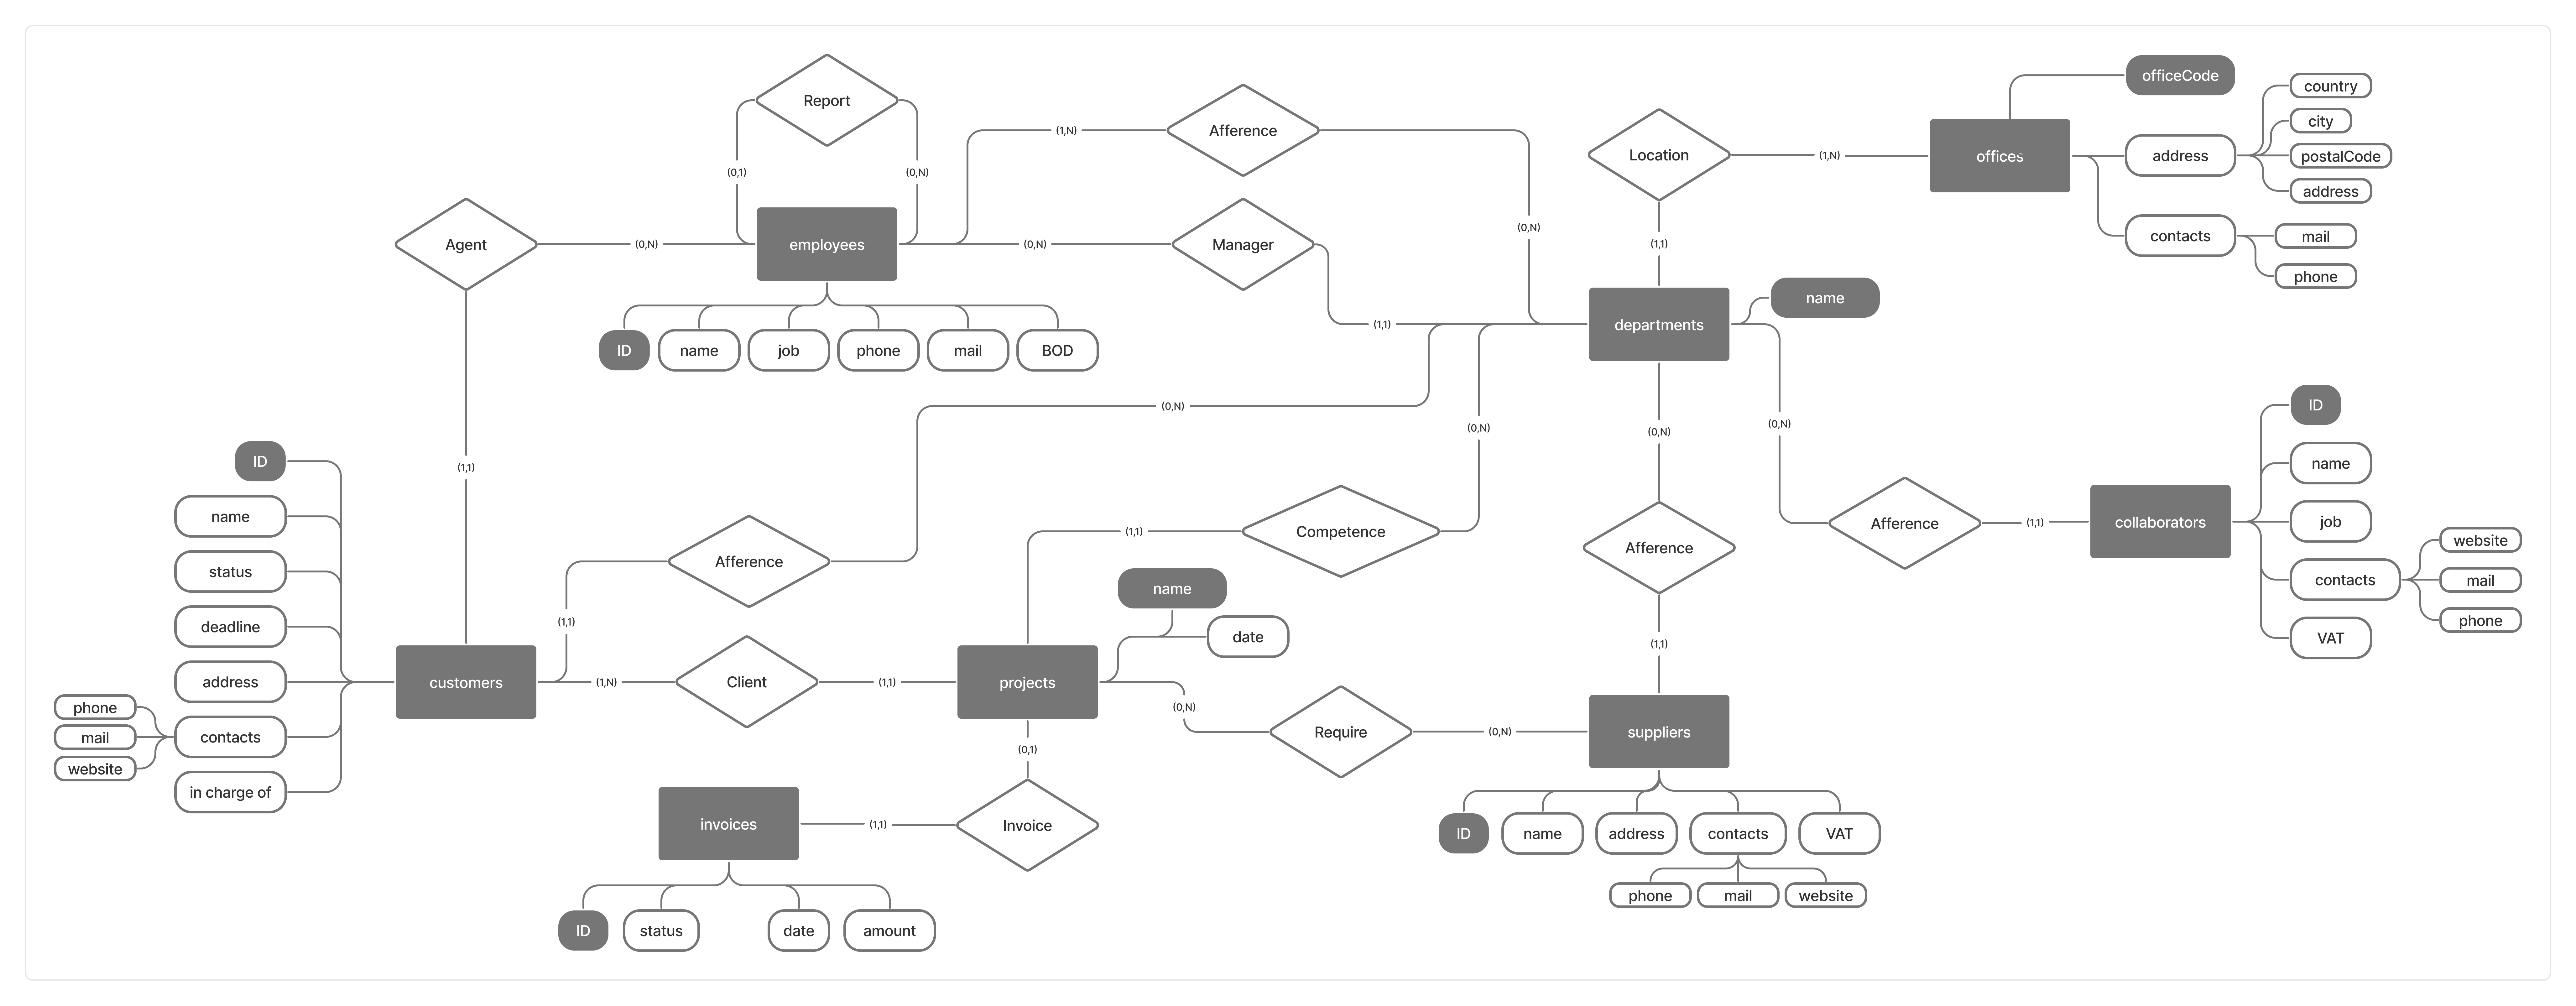
\includegraphics[width=0.9\columnwidth]{../../img/er_scheme_reviewed}
\end{center}

% NUOVO CAPITOLO 
\section{Schema Logico}\label{sec:schema-logico}
\begin{center}
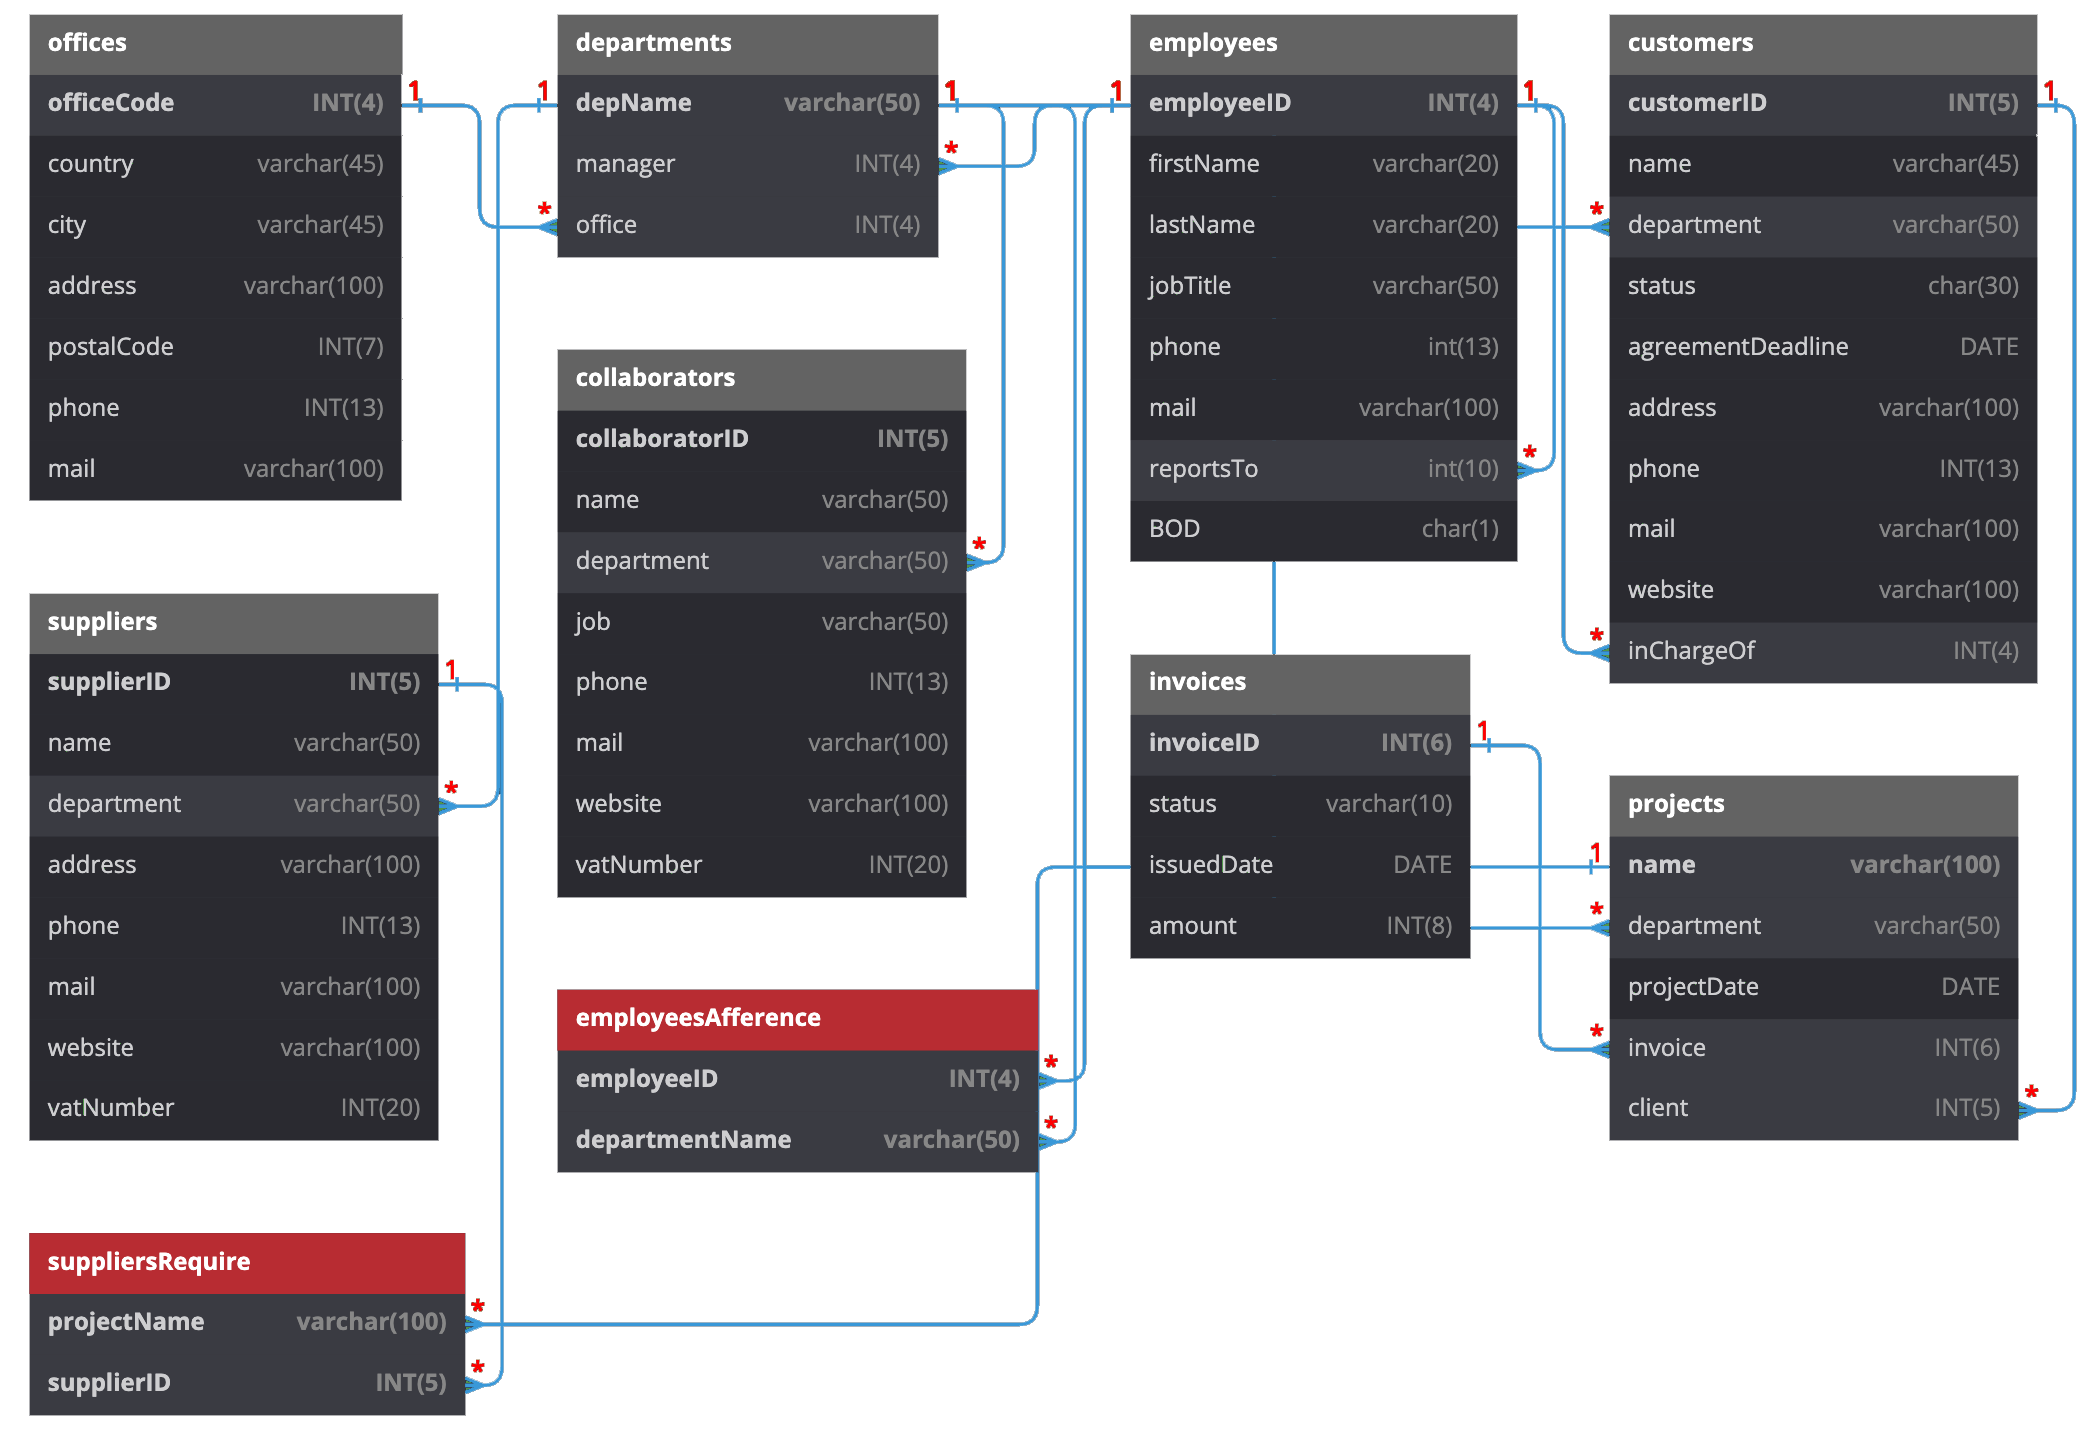
\includegraphics[width=0.9\columnwidth]{../../img/logic_scheme}
\end{center}
Nello schema logico ho voluto evidenziare le tabelle \textit{suppliersRequire} e \textit{employeeAfference} che ho dovuto implementare per realizzare le due relazioni molti a molti presenti nello schema Entity - Relationship.


% NUOVO CAPITOLO
\clearpage
\section{Progettazione Fisica}\label{sec:progettazione-fisica}
Per non appesantire troppo questo file ho voluto creare degli script SQL, rispettivamente per creare tabelle, view e store procedure e per riempire le tabelle, che possono esse scaricati dalla \href{https://github.com/enricolacchin/database-2023-final-project/}{\textbf{repo github}} del progetto oppure dai link sottostanti.
\begin{itemize}
\item File table\_creation.sql: \href{https://github.com/enricolacchin/database-2023-final-project/SQL/table_creation.sql}{\textbf{download}}
\item File view\_sp\_creation.sql: \href{https://github.com/enricolacchin/database-2023-final-project/SQL/view_sp_creation.sql}{\textbf{download}}
\item File data\_insert.sql: \href{https://github.com/enricolacchin/database-2023-final-project/SQL/data_insert.sql}{\textbf{download}}
\end{itemize}
Nella progettazione fisica voglio mettere l'attenzione sul controllo utilizzato per i vincoli non esprimibili citati in precedenza:
\flushleft
\begin{lstlisting}[language = SQL,label={lst:check}]
CREATE TABLE customers(
  /* ... */
  status char(30) CHECK(status IN ('Ongoing Negotiation', 'Agreed', 'In Progress', 'Done')),
  /* ... */
);
\end{lstlisting}
Tramite la keyword \textbf{CHECK} sono andato a controllare che quella determinata colonna facesse parte solamente di una lista definita.

\Sep \noindent
Per quanto riguarda le Stored Procedure la più interessante è quella che mi ritorna le fatture tra due date scelte.\\
Vengono fornite in input due date e tramite la keyword \textbf{BETWEEN} vado a estrapolare solamente le fatture richieste. Tramite le \textbf{JOIN} invece vado a rappresentare i dati in maniera più bella così da vedere anche il nome del cliente.
\begin{lstlisting}[language = SQL,label={lst:invoices-dates}]
CREATE PROCEDURE invoicesBetweenDates(IN startDate DATE, IN endDate DATE)
BEGIN
  SELECT customerID, customers.name, invoiceID, issuedDate FROM invoices
  INNER JOIN projects ON projects.invoice = invoices.invoiceID
  INNER JOIN customers ON customers.customerID = projects.client
  WHERE issuedDate BETWEEN startDate AND endDate;
END;
\end{lstlisting}


%----------------------------------------------
% FINE DOCUMENTO
%----------------------------------------------
\end{document}